%!Tex root = Report.tex
\Section{Evaluation}
\SubSection{Datasets}
As mentioned before datasets are generated using \texttt{networkx} library and there are two types of datasets, one sparse and two dense. Sparsity is measured based on the clustering coefficient of the graph. Sparse random graphs have a small clustering coefficient while the dense graphs have large clustering coefficient.\\
\\
We have created six groups of datasets each with two graph datasets with a fixed number of edges. One graph is a sparse graph while the other one is dense. Below is the table of all the datasets generated for testing.
\begin{table}[h]
\centering
	\begin{tabular}{|r|r|r|r|}
		\hline
		\multicolumn{1}{|c|}{Dataset} & \multicolumn{1}{c|}{Total Edges} & \multicolumn{1}{c|}{Dense (nodes)} & \multicolumn{1}{c|}{Sparse(nodes)} \\ \hline
		1                             & 20,000                           & 900                                & 2,000                              \\ \hline
		2                             & 50,000                           & 2,100                              & 5,000                              \\ \hline
		3                             & 100,000                          & 4,000                              & 9,500                              \\ \hline
		4                             & 200,000                          & 8,000                              & 19,000                             \\ \hline
		5                             & 500,000                          & 20,000                             & 47,000                             \\ \hline
		6                             & 1,000,000                        & 40,000                             & 91,000                             \\ \hline
	\end{tabular}
\end{table}

\begin{figure}
	\centering
	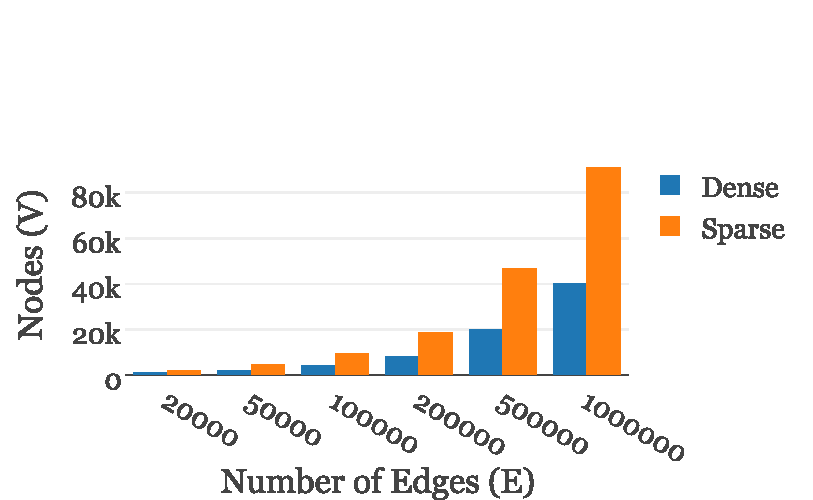
\includegraphics[scale=0.7, trim = 0 0 20 0]{Graphs/dataset-stats.pdf}
	\caption{Dataset Statistics \label{fig:datasets}}
\end{figure}

The \textbf{average degree distribution} for the sparse graph is 12 edges/node while for dense graph is 25 edges/node.
\SubSection{Setup}
The following are the set of machines used for evaluation: 
\begin{itemize}
	\item
	Neo4j: Amazon EC2 instance with 4 vCPUs and 7.5GB memory with 20GB disk space.
	\item
	GraphLab: Amazon EC2 instance with 4 vCPUs and 7.5GB memory with 20GB disk space.
\end{itemize}
\SubSection{Evaluation Measure}
All the above datasets are run on both Neo4j and GraphLab systems and performance evaluation is done using \textbf{Execution Time}. Time of execution is calculated starting from the beginning of the clustering algorithm till the end. \\
Execution time does not include the time taken for the dataset to load into the database systems. On an another note, GraphLab is a graph processing system which loads the dataset into memory and is really quick, for example, a dataset of 100,000 edges takes around 5 seconds to load into memory, whereas Neo4j stores each node in its database on a persistent storage. Therefore it takes quite a long time as compared to GraphLab.